\section{Diseño e implementación}
\setcounter{sectiontotal}{3}

% TODO Agregar lo de los ECA!
% TODO mejorar esta imagen
\begin{frame}
\frametitle{\pagetitle}
\framesubtitle{Flujo de interacción}
\centering
\begin{overprint}
\onslide<1|handout:1> 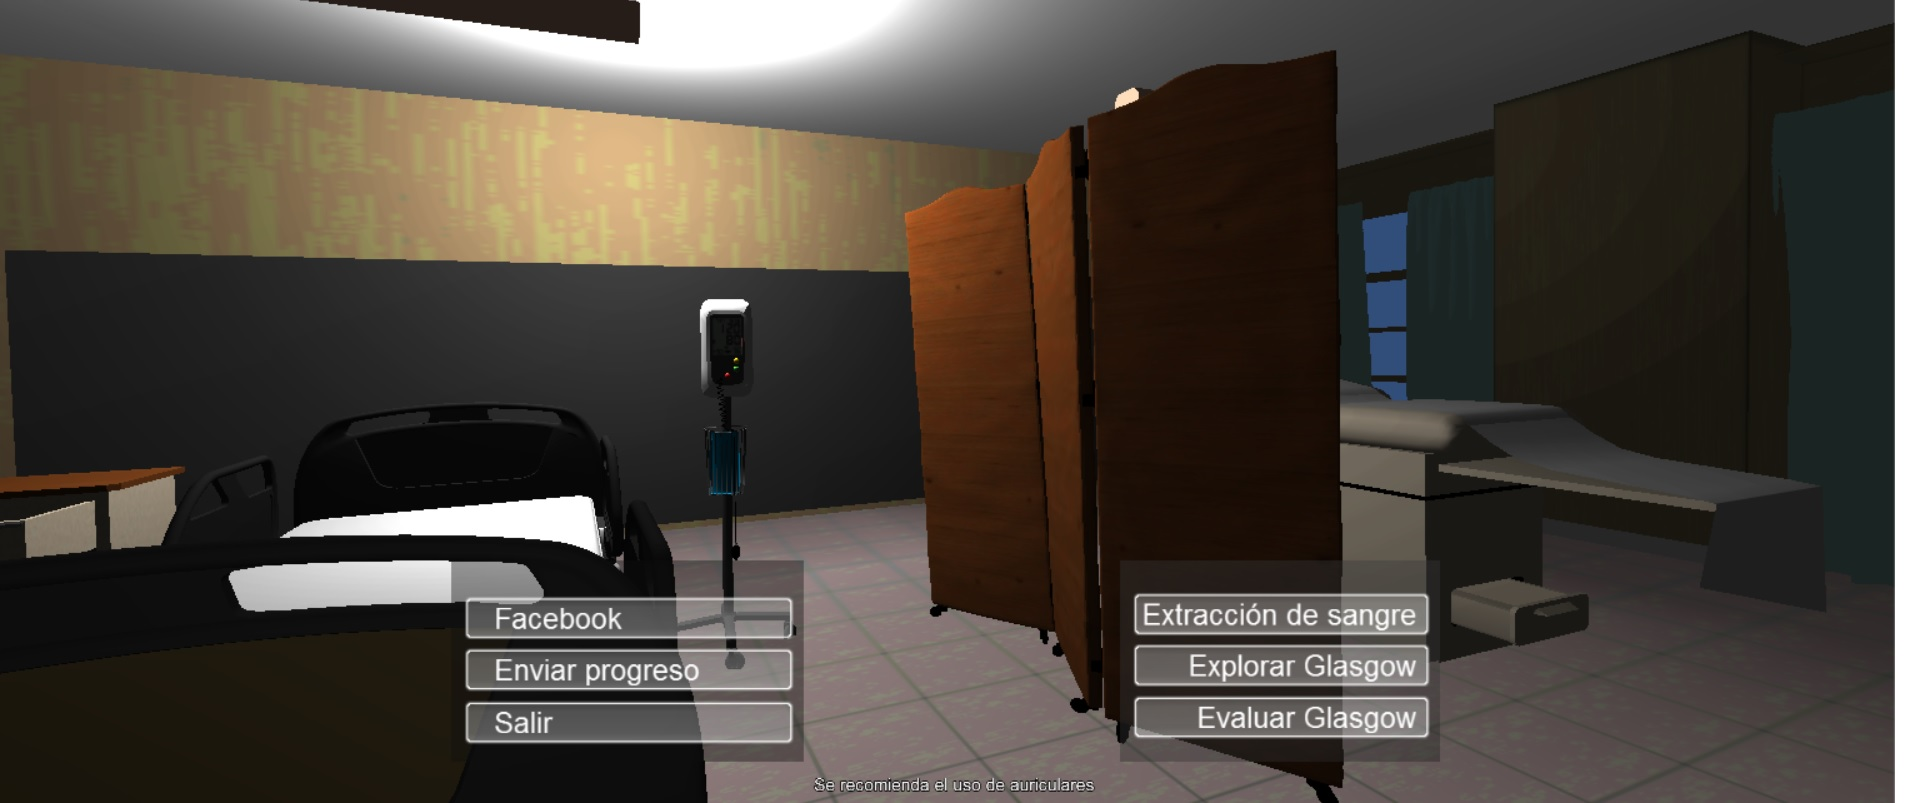
\includegraphics[width=\textwidth]{../solucion/images/pantalla_inicio.jpg} 
\onslide<2|handout:0> 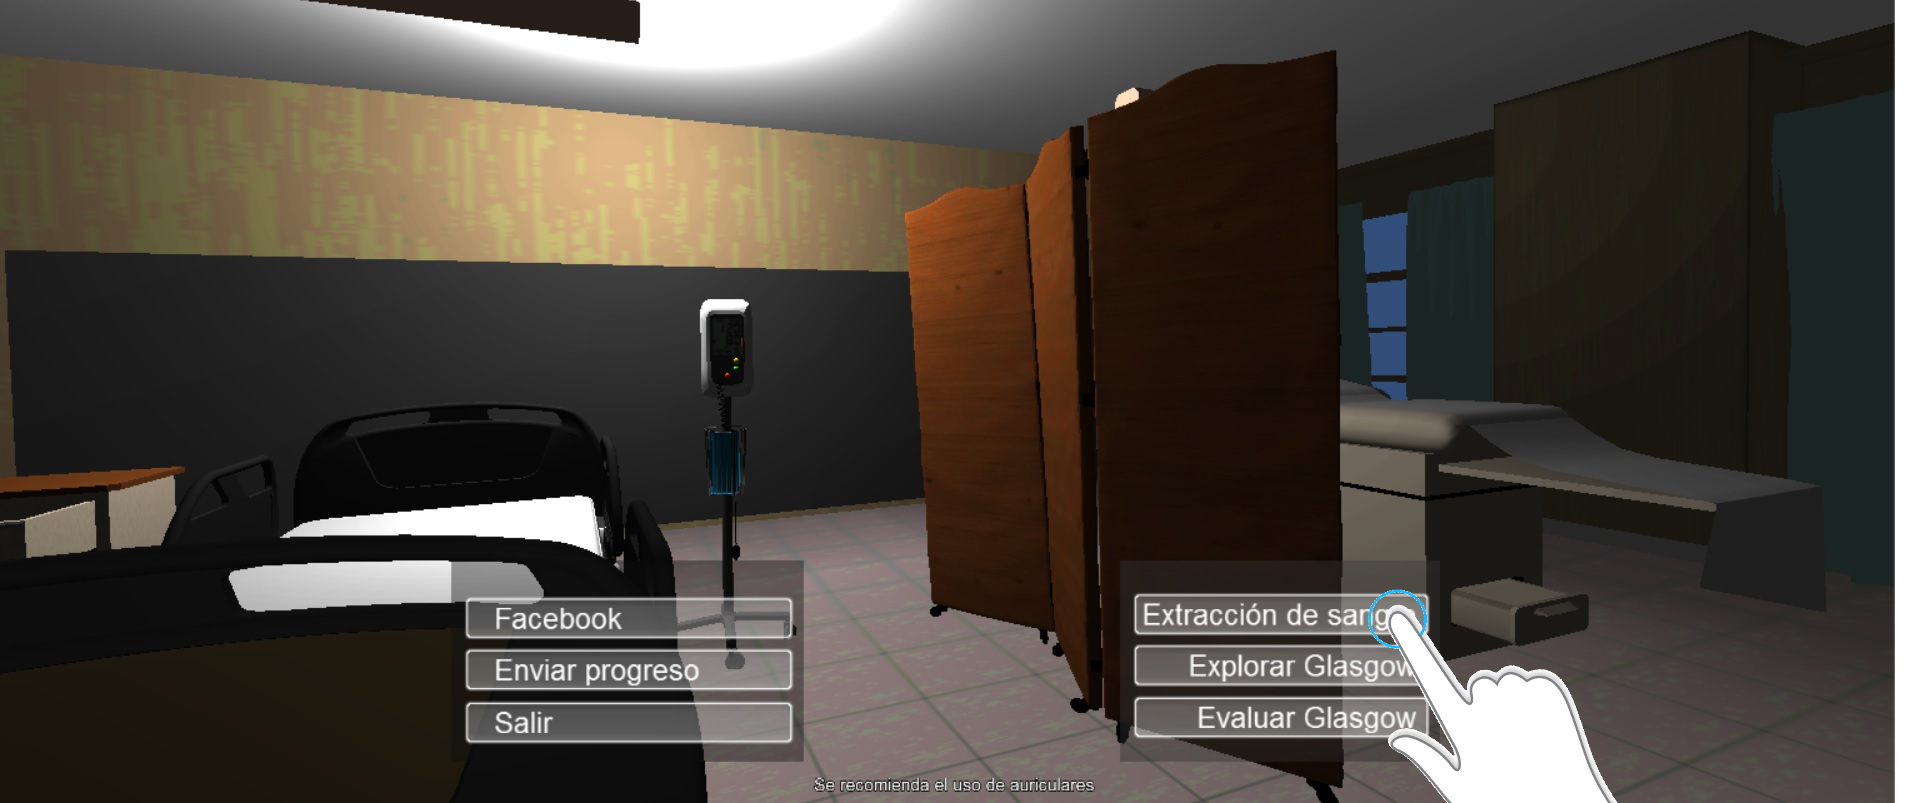
\includegraphics[width=\textwidth]{imagenes/flujo/flujo2.png} 
\onslide<3|handout:0> 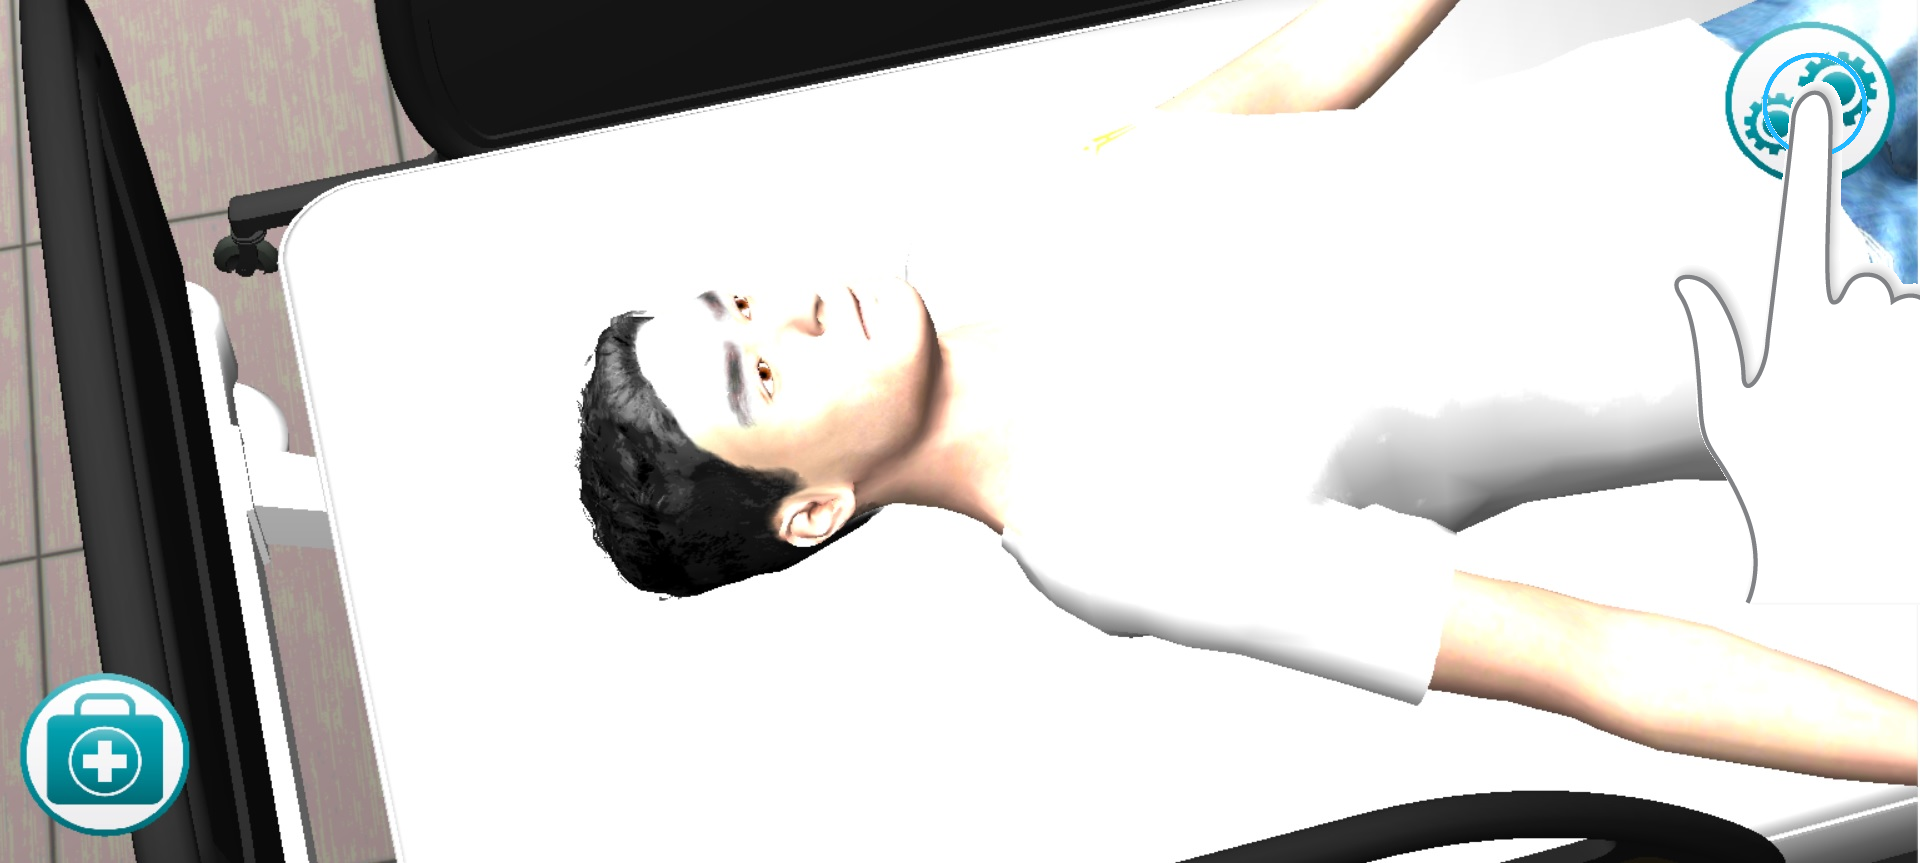
\includegraphics[width=\textwidth]{imagenes/flujo/flujo3.png} 
\onslide<4|handout:0> 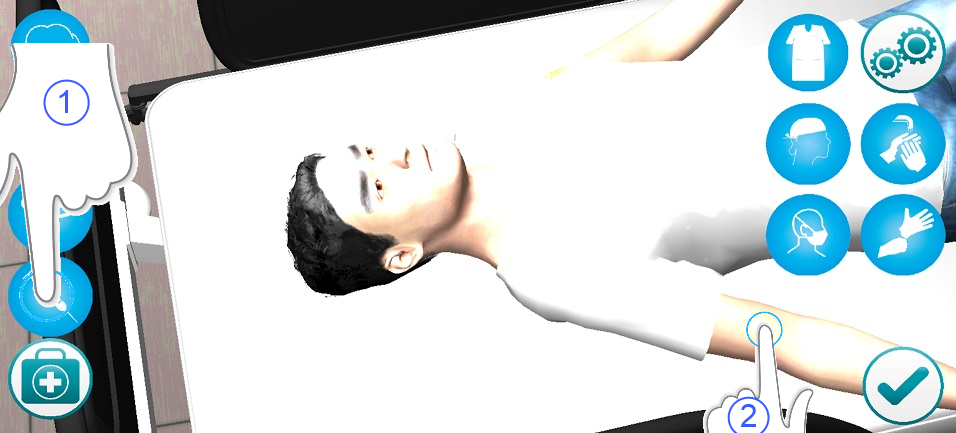
\includegraphics[width=\textwidth]{imagenes/flujo/flujo4.png} 
\onslide<5|handout:0> 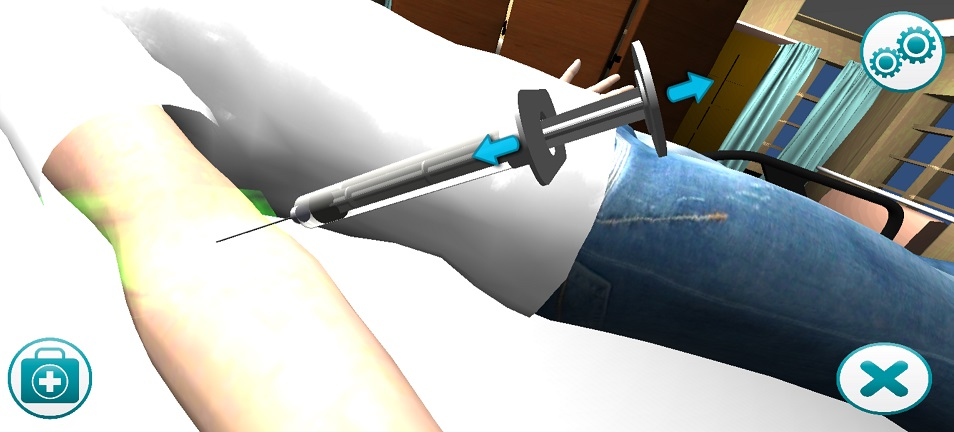
\includegraphics[width=\textwidth]{../solucion/images/hemocultivo_jeringa_ampliada.jpg} 
\onslide<6|handout:0> 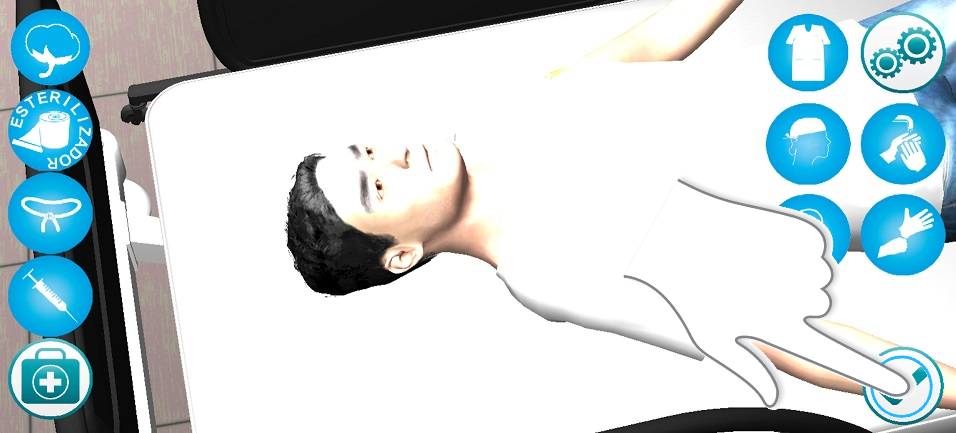
\includegraphics[width=\textwidth]{imagenes/flujo/flujo6.png} 
\onslide<7|handout:0> 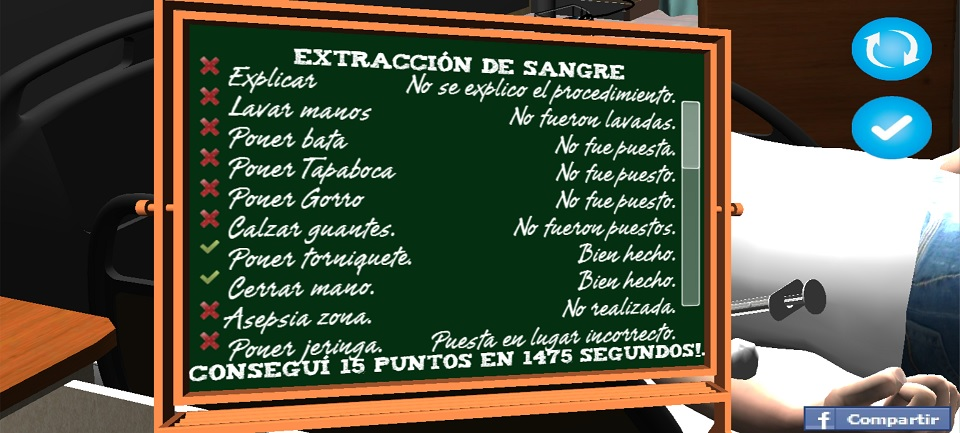
\includegraphics[width=\textwidth]{../solucion/images/resultado_hemocultivo.jpg}
\onslide<8|handout:0> 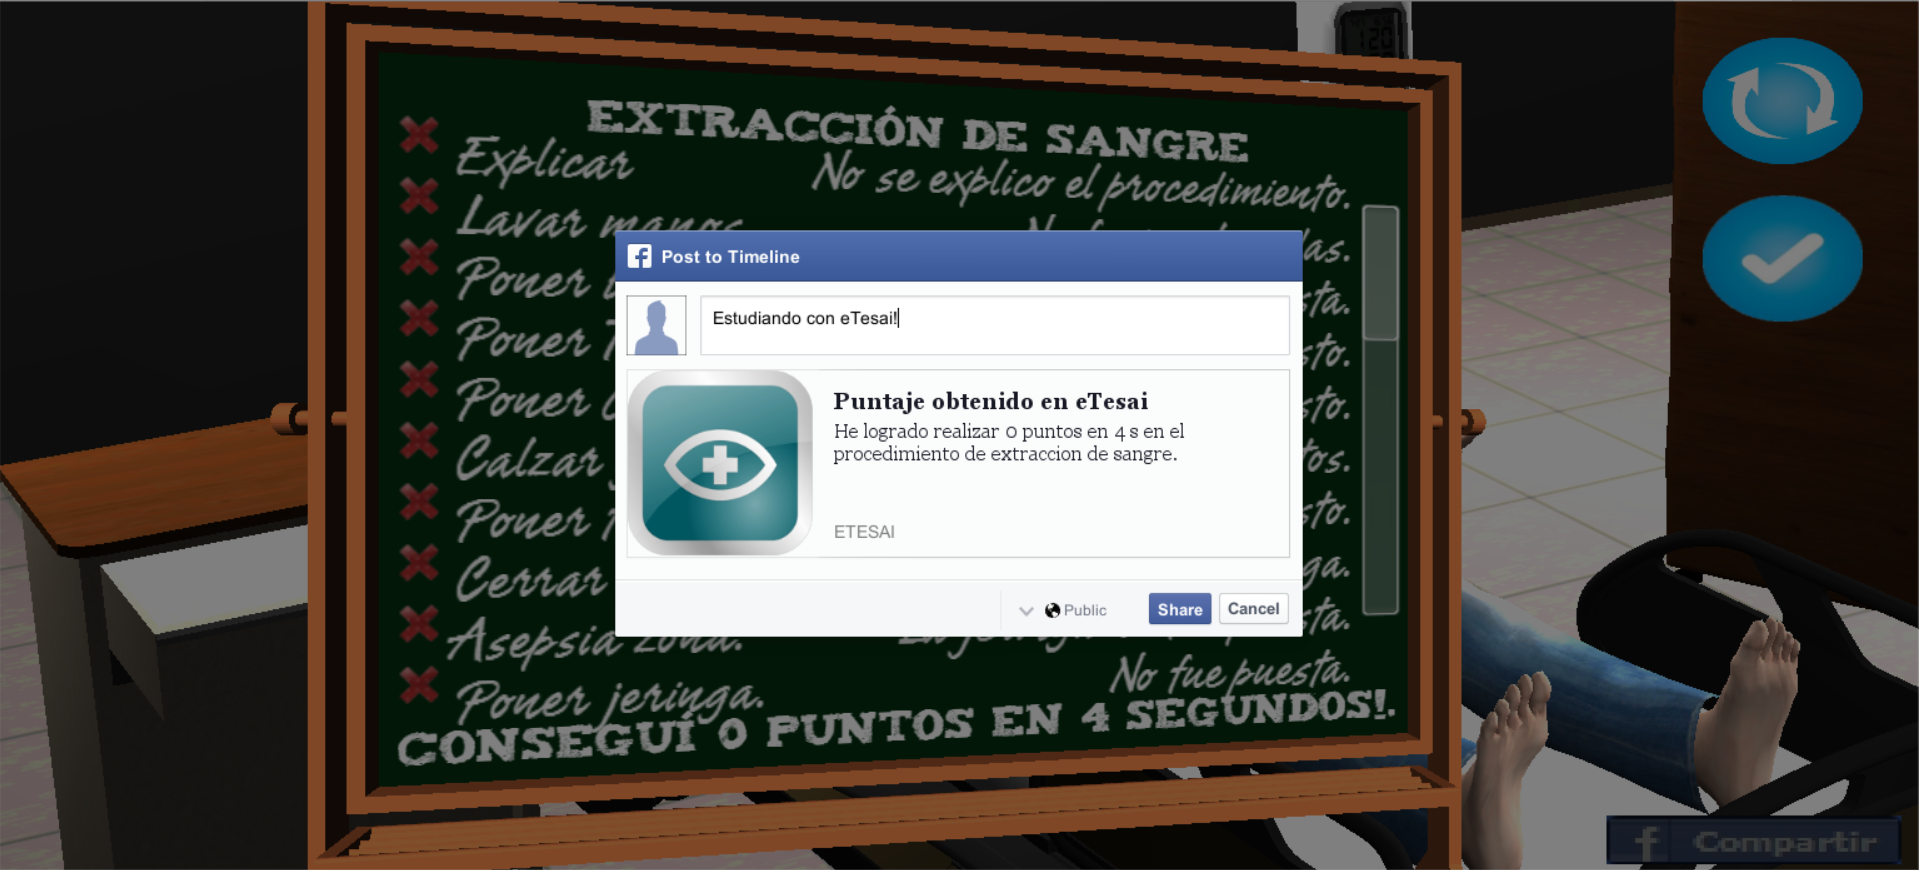
\includegraphics[width=\textwidth]{imagenes/flujo/flujo18.png} 
\onslide<9|handout:0> 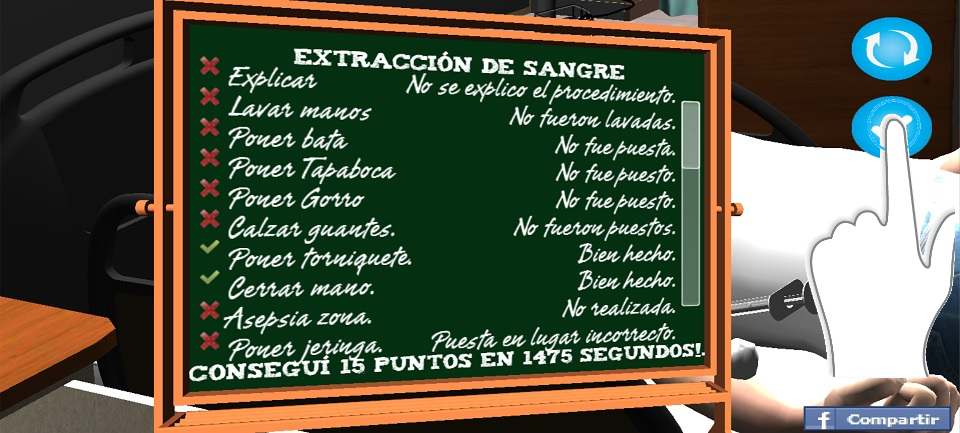
\includegraphics[width=\textwidth]{imagenes/flujo/flujo8.png} 
% Glasgow
\onslide<10|handout:0> 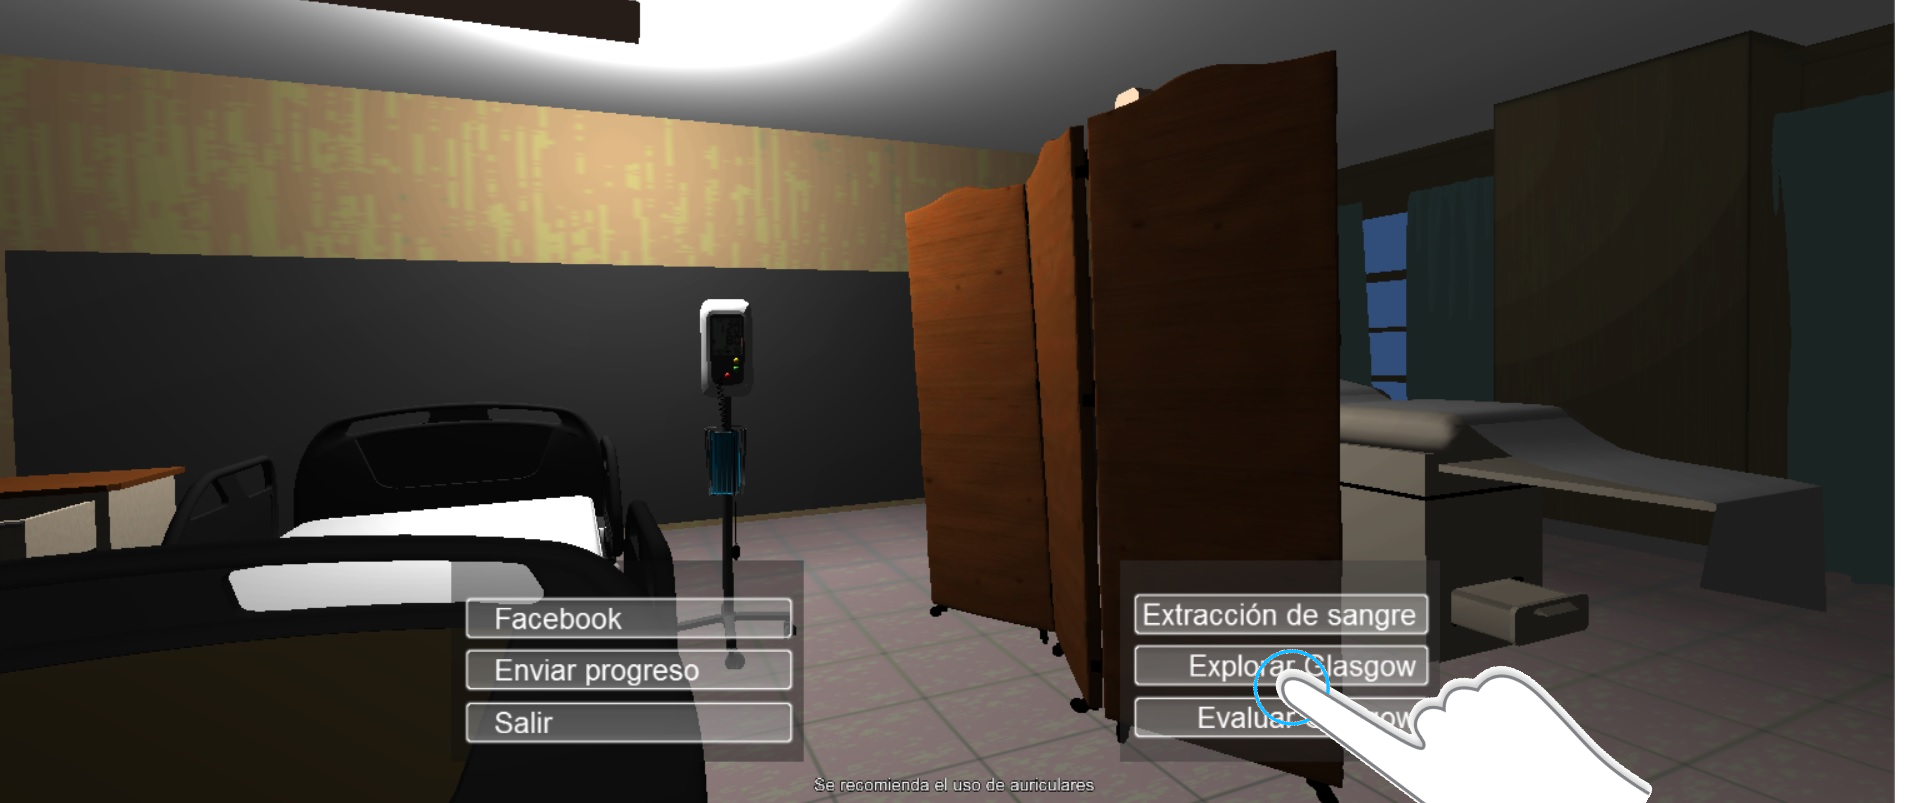
\includegraphics[width=\textwidth]{imagenes/flujo/flujo9.png}
\onslide<11|handout:0> 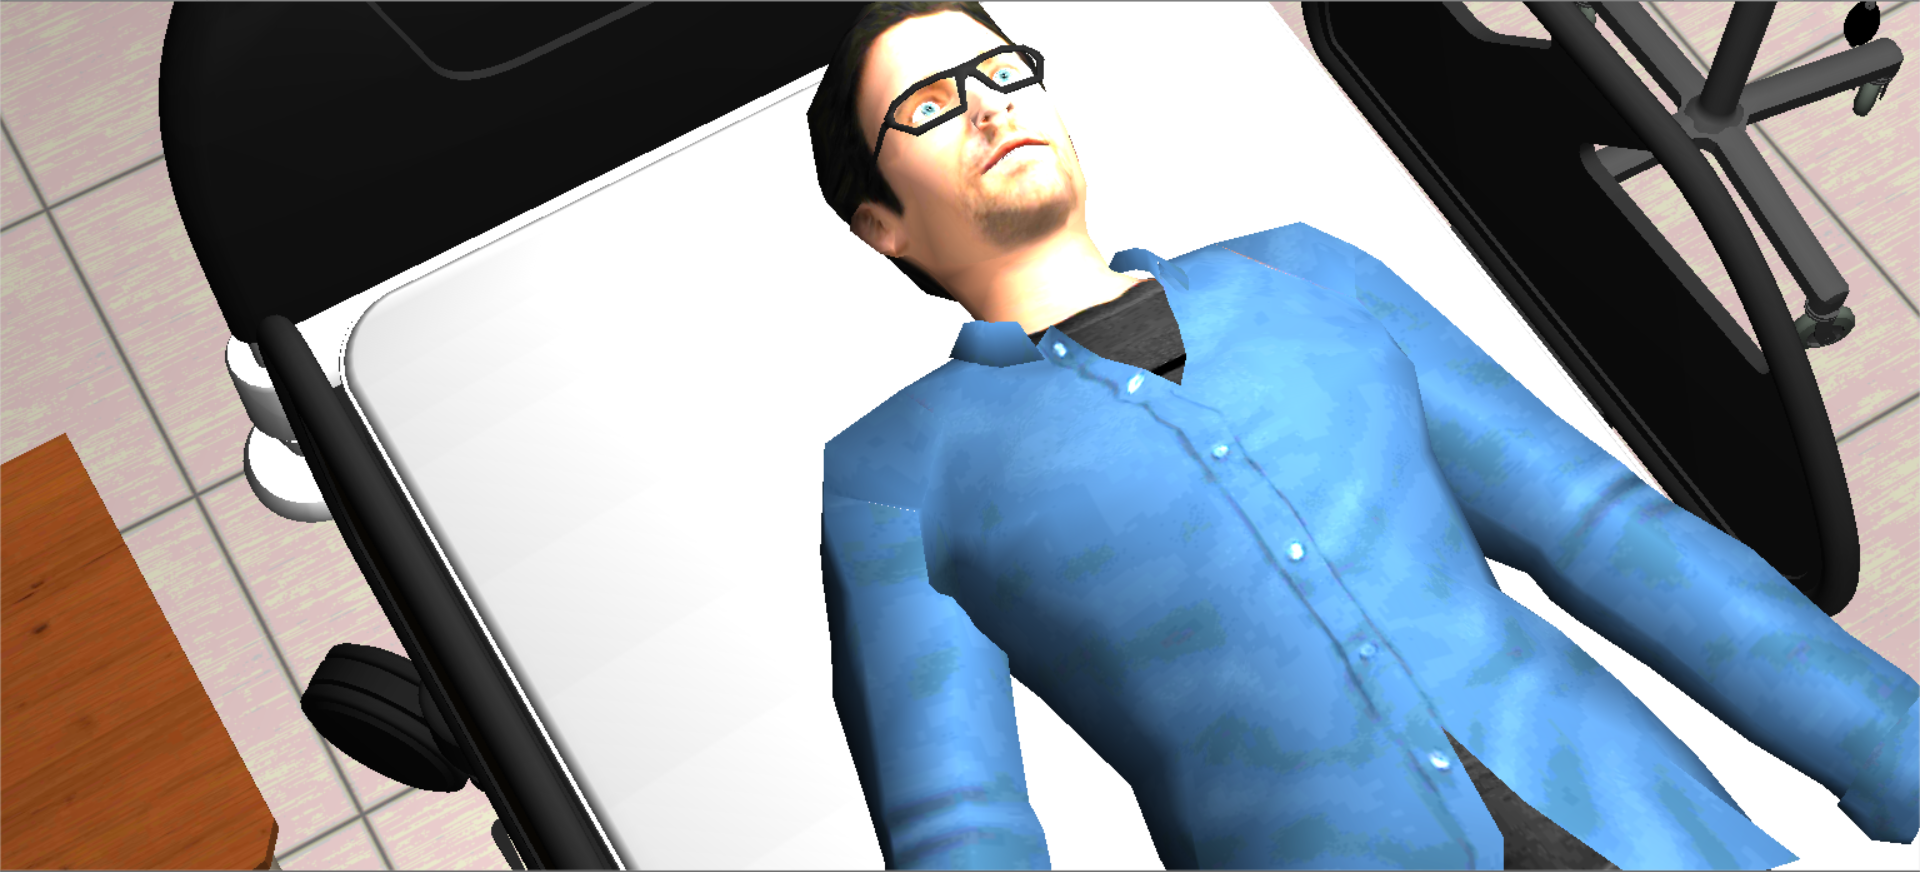
\includegraphics[width=\textwidth]{imagenes/flujo/flujo10.png}
%\onslide<12|handout:0> 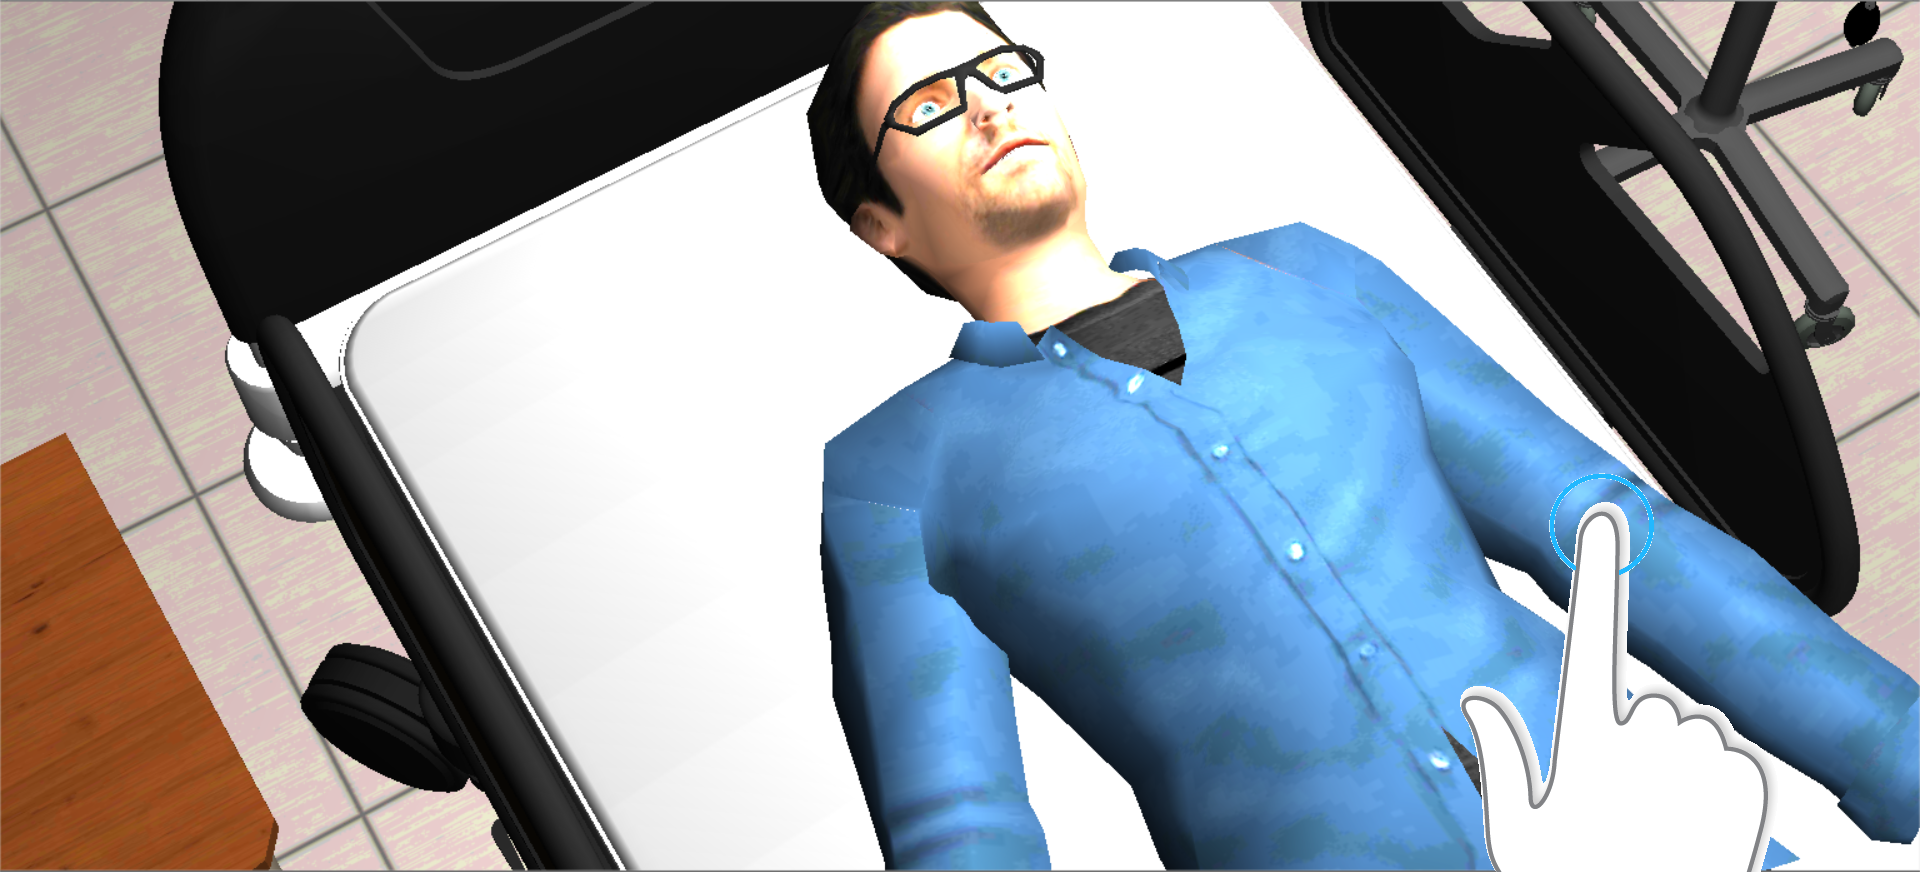
\includegraphics[width=\textwidth]{imagenes/flujo/flujo11.png}
\onslide<12|handout:0> 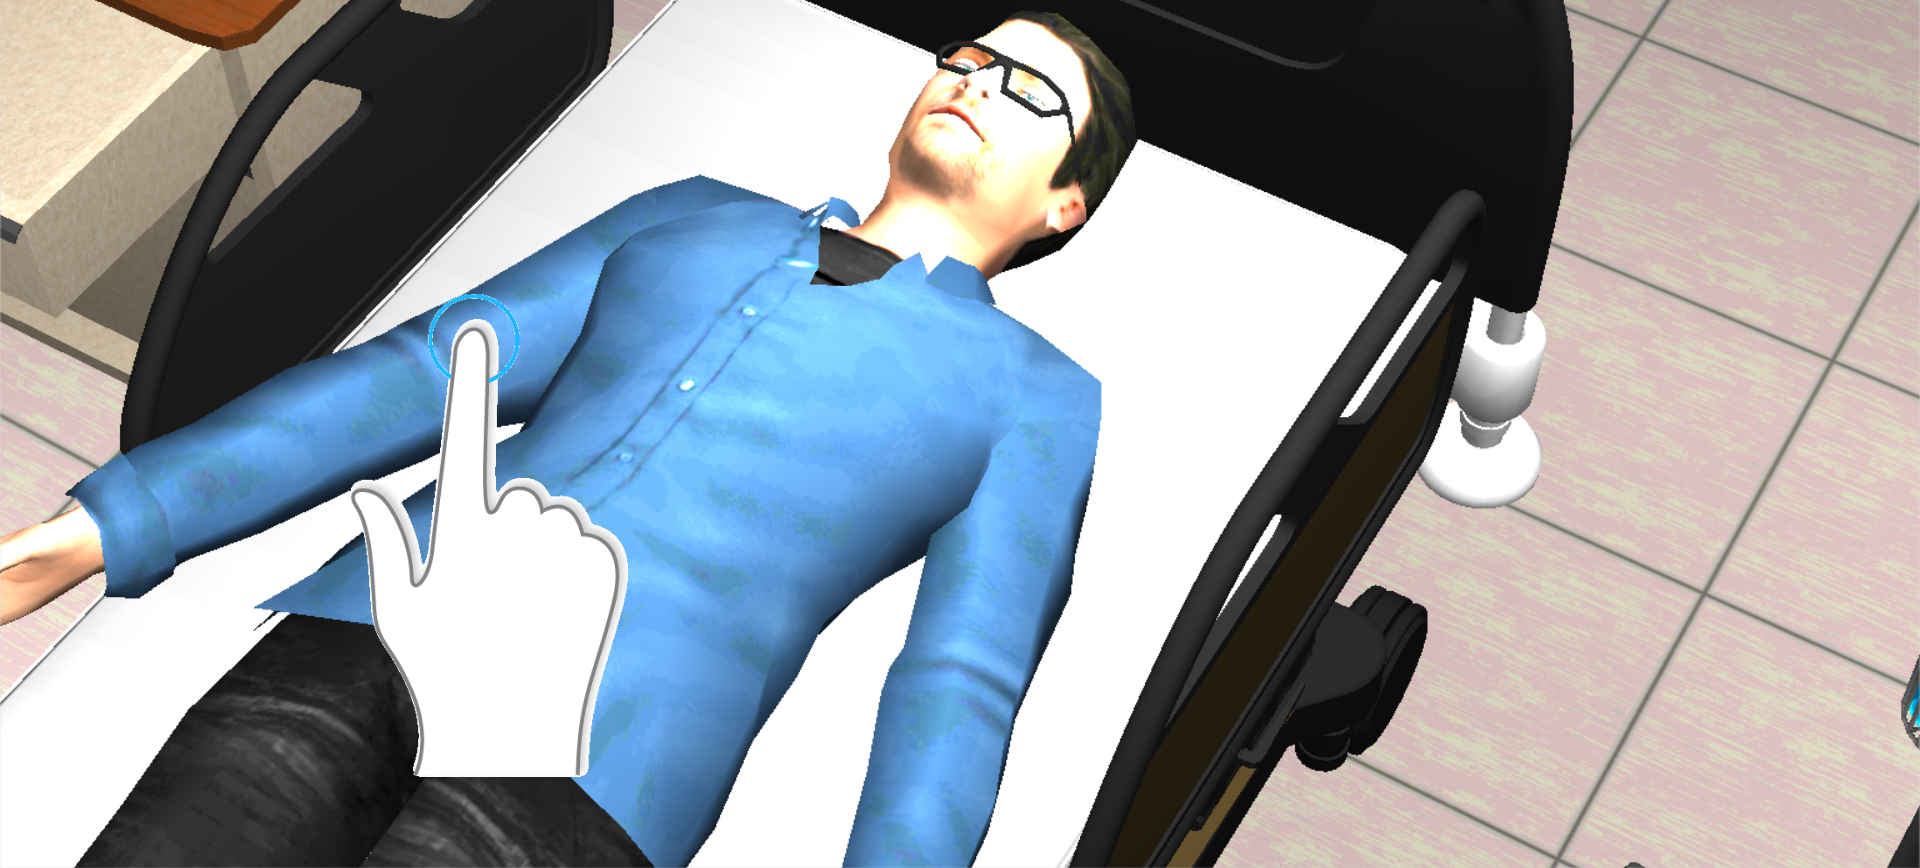
\includegraphics[width=\textwidth]{imagenes/flujo/flujo12.png}
\onslide<13|handout:0> 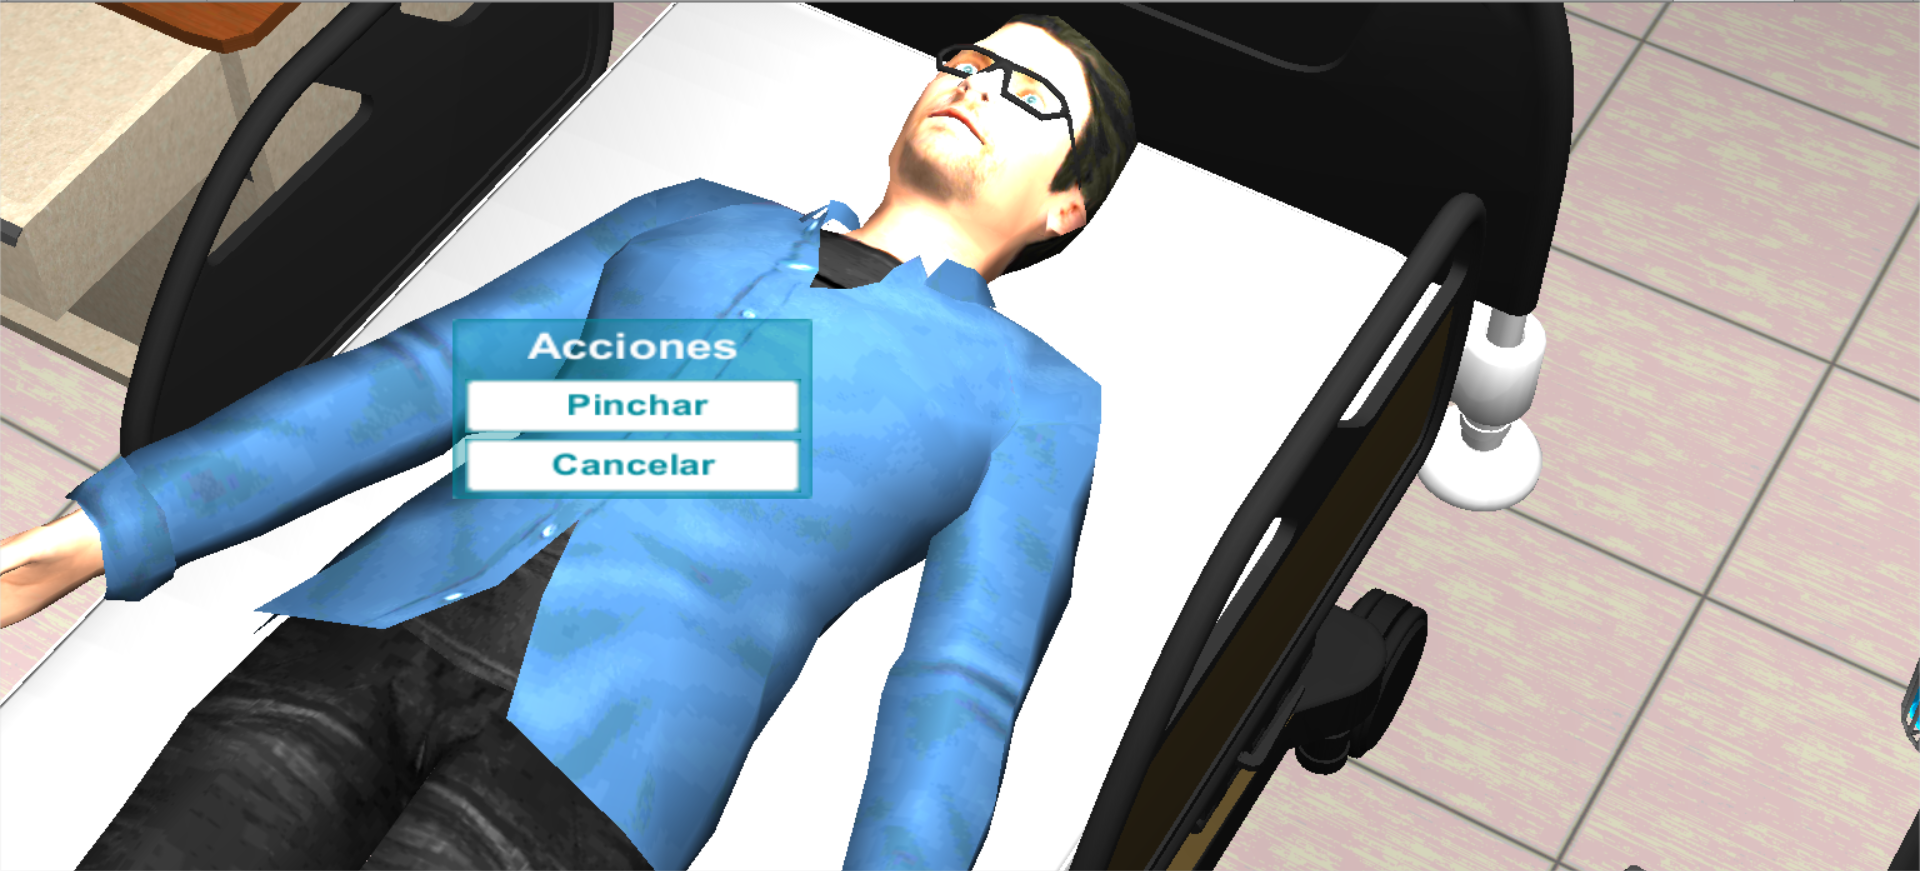
\includegraphics[width=\textwidth]{imagenes/flujo/flujo13.png}
\onslide<14|handout:0> 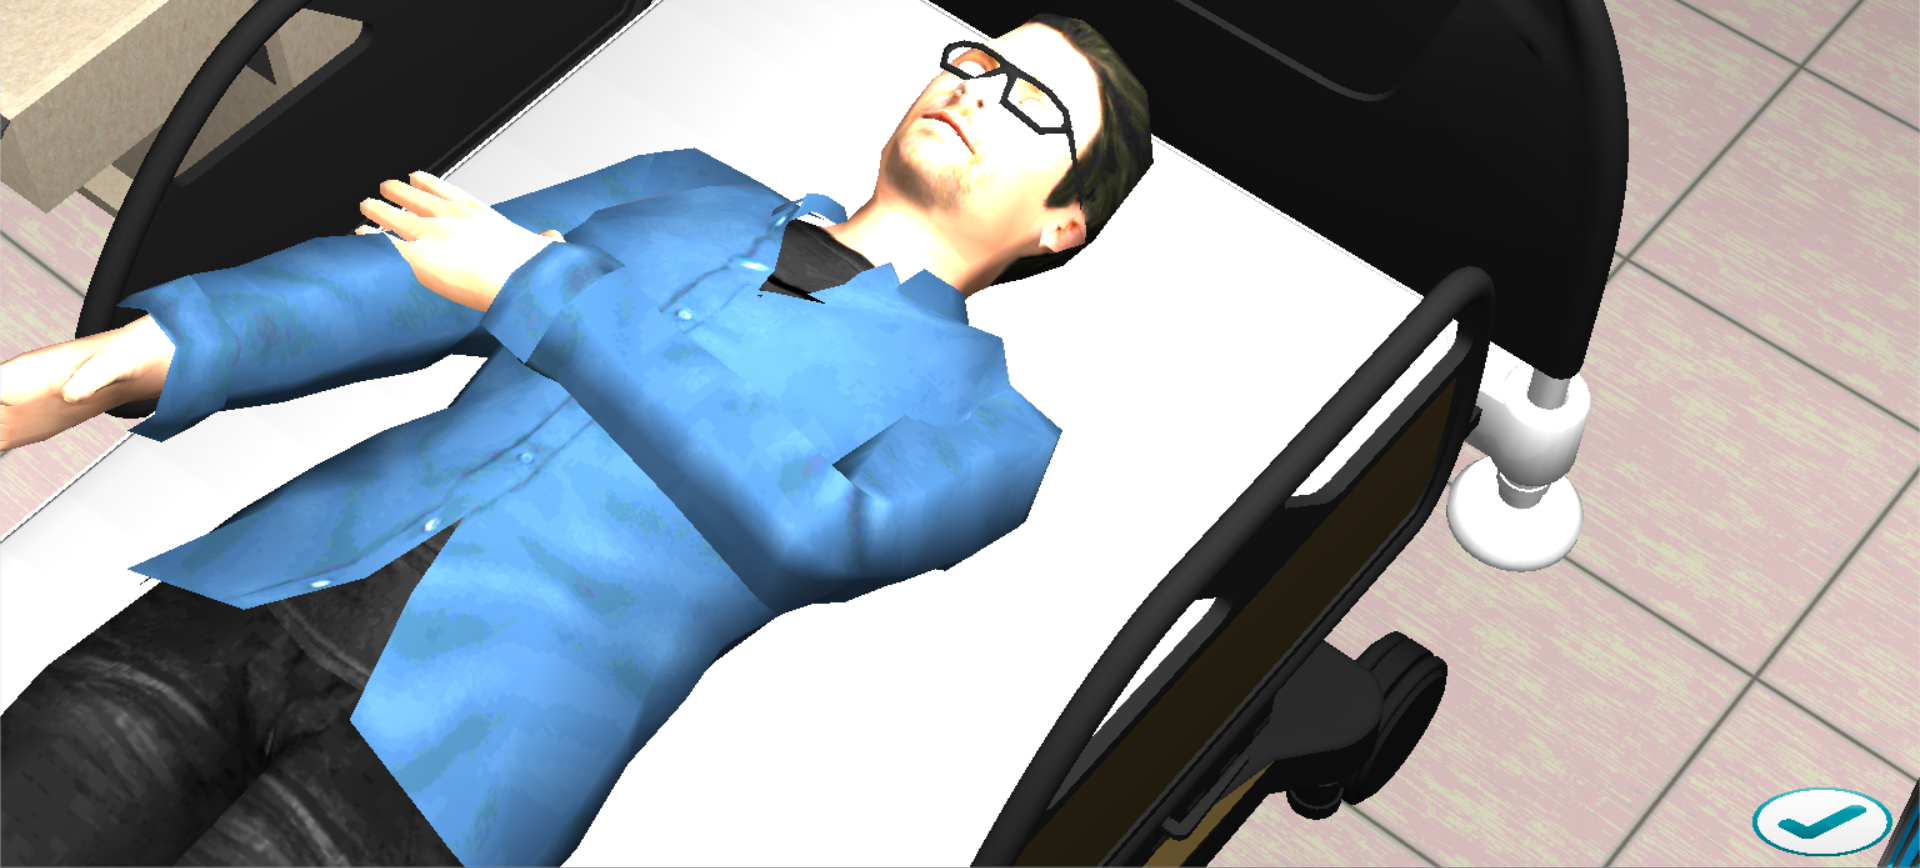
\includegraphics[width=\textwidth]{imagenes/flujo/flujo14.png}
\onslide<15|handout:0> 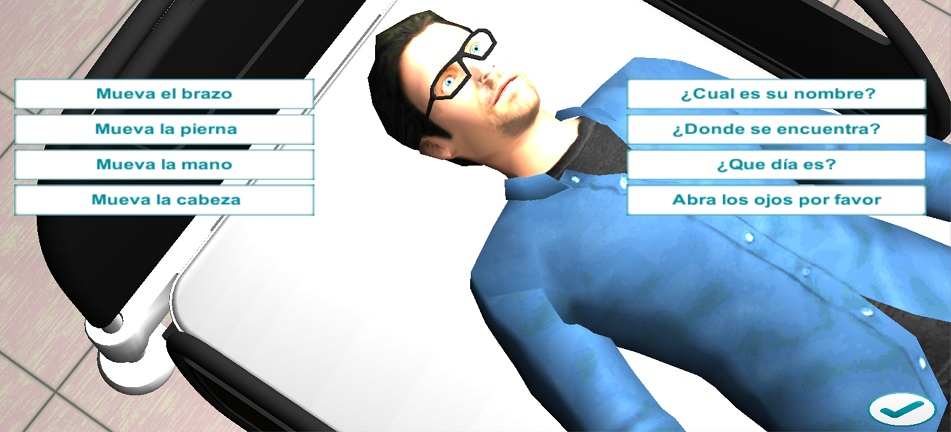
\includegraphics[width=\textwidth]{../solucion/images/glasgow_comandos_voz.jpg}
\onslide<16|handout:0> 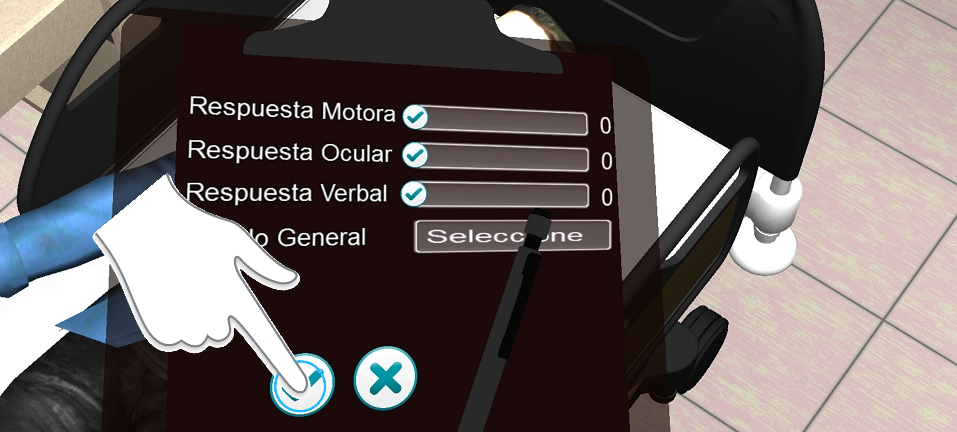
\includegraphics[width=\textwidth]{imagenes/flujo/flujo16.png}
\onslide<17|handout:0> 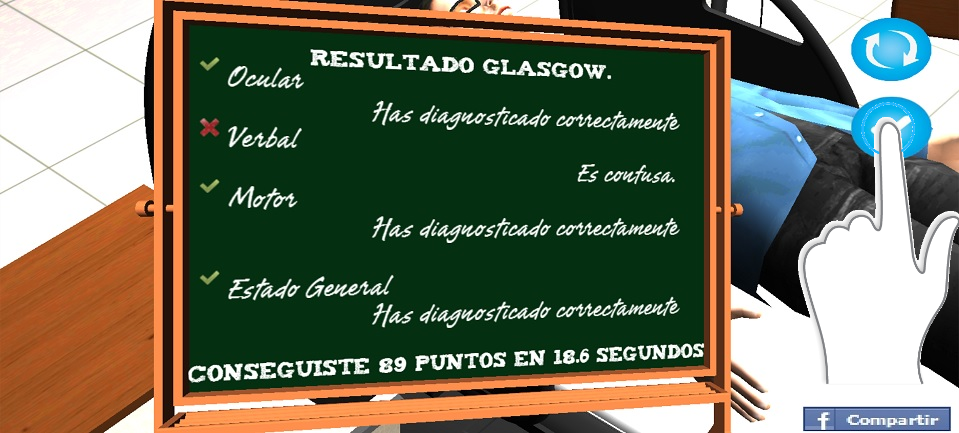
\includegraphics[width=\textwidth]{imagenes/flujo/flujo17.png}





\end{overprint}
\end{frame}
